\section{CPU Arichitecture}
\label{sec:cpu_memory}

\noindent
This section provides a high-level overview of the CPU to provide context/motivation for the following algorithms and data structures.

\begin{Def}[Central Processing Unit (CPU)]

    The \textbf{CPU (Central Processing Unit)}, is a hardware component that \emph{computes} instructions within a computer.
    Abstract models that define interfaces between hardware and software for a CPU are called \textbf{instruction set architectures (ISA)}.
    
    Possible operations are detailed as \textbf{opcodes} (operation codes), which are numeric identifiers for each instruction. 
    Moreover, the ISA defines supported data types, \textbf{registers (temporary storage locations)}, and addressing modes (ways to access memory).\\

    \noindent
    ISA's are defines the instruction set, which allows for flexibility in hardware performance needs. This various categories:
    \begin{itemize}
        \item \textbf{CISC (Complex Instruction Set Computing):} Large number of complex instructions (multiple operations per instruction).
        \item \textbf{RISC (Reduced Instruction Set Computing):} Small set of simple/efficient instructions.
        \item \textbf{VLIW (Very Long Instruction Word):} Enables instruction parallelism (simultaneous execution).
        \item \textbf{EPIC (Explicitly Parallel Instruction Computing):} More explicit control over parallel execution.
    \end{itemize}
    \noindent
    Smaller more theoretical architectures exists such as \textbf{MISC (Minimal Instruction Set Computing)} and \textbf{OISC (One Instruction Set Computing)}, which are not used in practice.
    Popular CPU architectures include x86\_64, and ARM64 (64-bit), originating from x86 and ARM (32-bit). 
    
    The implementation of a CPU on a circuit board is called a \textbf{microprocessor}. Multiple CPUs on a single circuit board are \textbf{multi-core processors}, where each \emph{core}
    is a fully functional CPU.
\end{Def}

\newpage
\begin{Def}[CPU Anatomy: Von Neumann Architecture]

    Modern computers operate on the \textbf{Von Neumann architecture}, which consists of three primary components:
    \begin{itemize}
        \item \textbf{ALU (Arithmetic Logic Unit):} Performs arithmetic and logical operations (e.g., addition, subtraction, AND, OR).
        \item \textbf{Control Unit (CU):} Directs the operation of the CPU, fetching and decoding instructions, and controlling the flow of data.
        \item \textbf{Memory Unit (MU):} Manages data storage and retrieval, including registers and cache memory.
    \end{itemize}
    \noindent
    All these components have volatile memory, lost when the computer is turned off.
\end{Def}

\begin{Def}[CPU Execution Flow]
    
    \label{def:cpu_execution_flow}

    The \textbf{CPU execution flow} is the sequence of operations that the CPU performs to execute a program. 
    It typically follows these steps:
    \begin{enumerate}
        \item \textbf{Fetch:} Fetches the next instruction from memory.
        \item \textbf{Decode:} Decodes the fetched instruction to associated opcode and operands.
        \item \textbf{Execute:} Perform decoded operation using the ALU or other components.
        \item \textbf{Store:} Save results of the operation back into memory or registers.
    \end{enumerate}
    \noindent
    This cycle is repeated until the program completes or an interrupt occurs.
\end{Def}

\begin{Def}[Registers]

    \label{def:registers}

    \textbf{Registers} are small, high-speed storage locations within the CPU that hold data temporarily during execution. 
    Common types of registers include:
    \begin{itemize}
        \item \textbf{General-Purpose Registers (GPR):} Hold general data storage and manipulation.
        \item \textbf{Special-Purpose Registers:} For specific functions, such as a reference to the current line of code.
        \item \textbf{Floating-Point Registers:} Floating-point arithmetic (e.g., decimal numbers).
    \end{itemize}
    \noindent
    Registers are faster than main memory (RAM) and are used to store frequently accessed data during program execution.
\end{Def}

\newpage

\noindent
The following is an example of the primary registers in the x86-32 (IA-32) architecture, which is a CISC architecture.
\begin{table}[h]
\centering
\begin{tabular}{|l|c|l|}
\hline
\textbf{Register} & \textbf{Size} & \textbf{Purpose} \\
\hline
EAX    & 32-bit & Accumulator (arithmetic / return value) \\
EBX    & 32-bit & Base register (data pointer)            \\
ECX    & 32-bit & Counter (loops, shifts)                 \\
EDX    & 32-bit & Data register (I/O, multiply/divide)    \\
ESI    & 32-bit & Source index (string / memory ops)      \\
EDI    & 32-bit & Destination index (string / memory ops) \\
EBP    & 32-bit & Base/frame pointer (stack-frame anchor) \\
ESP    & 32-bit & Stack pointer                           \\
EIP    & 32-bit & Instruction pointer (program counter)   \\
EFLAGS & 32-bit & Flags / status register (ZF, CF, OF…)   \\
\hline
\end{tabular}
\caption{Primary registers of the x86-32 (IA-32) architecture. \textbf{Note:} Registers are prefixed with \underline{`E' for 32-bit, `R' for 64-bit in x86-64}.}
\end{table}


\begin{Def}[Machine Code \& Compilation]

    \label{def:machine_code}

    Code is separated into two main areas of memory management, the program itself, and the data in transit during execution.
    The program itself is broken up such as follows:
    \begin{itemize}
        \item \textbf{Text Segment:} The part of the program which contains the executable code.
        \item \textbf{Data Segment:} The part of the program which contains global and static variables.
        \item \textbf{Machine Code:} The compiled code of the program, which is executed by the CPU.
    \end{itemize}

    \noindent
    Once the code compiles, our data segment is further divided into two parts in memory:
    \begin{itemize}
        \item \textbf{Initialized Data:}  Data given a value before the program starts (global variables).
        \item \textbf{Uninitialized Data:} Data yet to be assigned (local variables), which are zeroed at program start.
    \end{itemize}
    \noindent
    By memory we mean the \textbf{RAM (Random Access Memory)} hardware component, which stores temporary data, constantly 
    communicating with the CPU or external storage (e.g., hard drive, SSD). Each memory cell is IDed by a unique monotonic \textbf{address},
    often in hexadecimal format(e.g., 0xF00, 0xF01, etc).
\end{Def}

\newpage 

\begin{Def}[Operating System (OS)]

    \label{def:operating_system}

    Implemented ISAs only provide an interface to the CPU; Programmers must
    design how their systems utilize the CPU (e.g., file and memory management), such software is called an \textbf{operating system (OS)}.
\end{Def}

\vspace{-1em}
\begin{Tip} In an analogous sense, say we have a train riding service. The ISA would be the specifications of the trains, rails, routes, and stations needed.
    The physical implementation of trains, rails, and stations would be the CPU. The OS would be the train schedule system, managing external 
    factors such as workers and other tasks effecting the train service.
\end{Tip}

\begin{Def}[The Kernel]

    \label{def:kernel}

    The \textbf{kernel} is a \textbf{process} (a program) vital for OS operation, always running with the highest 
    priority. It is the only program that can directly interact with the CPU and various hardware components.

    Other processes running on the system are called \textbf{user processes}. This is where applications and other user-level programs 
    run. If a user wishes to perform a task that requires hardware access (e.g., writing/reading files), they must request the kernel called a \textbf{system call (syscall)}. System 
    calls provide an \textbf{Application Programming Interface (API)} for user processes to interact with the kernel.
\end{Def}

\vspace{-1em}
\begin{figure}[ht!]
    \centering
    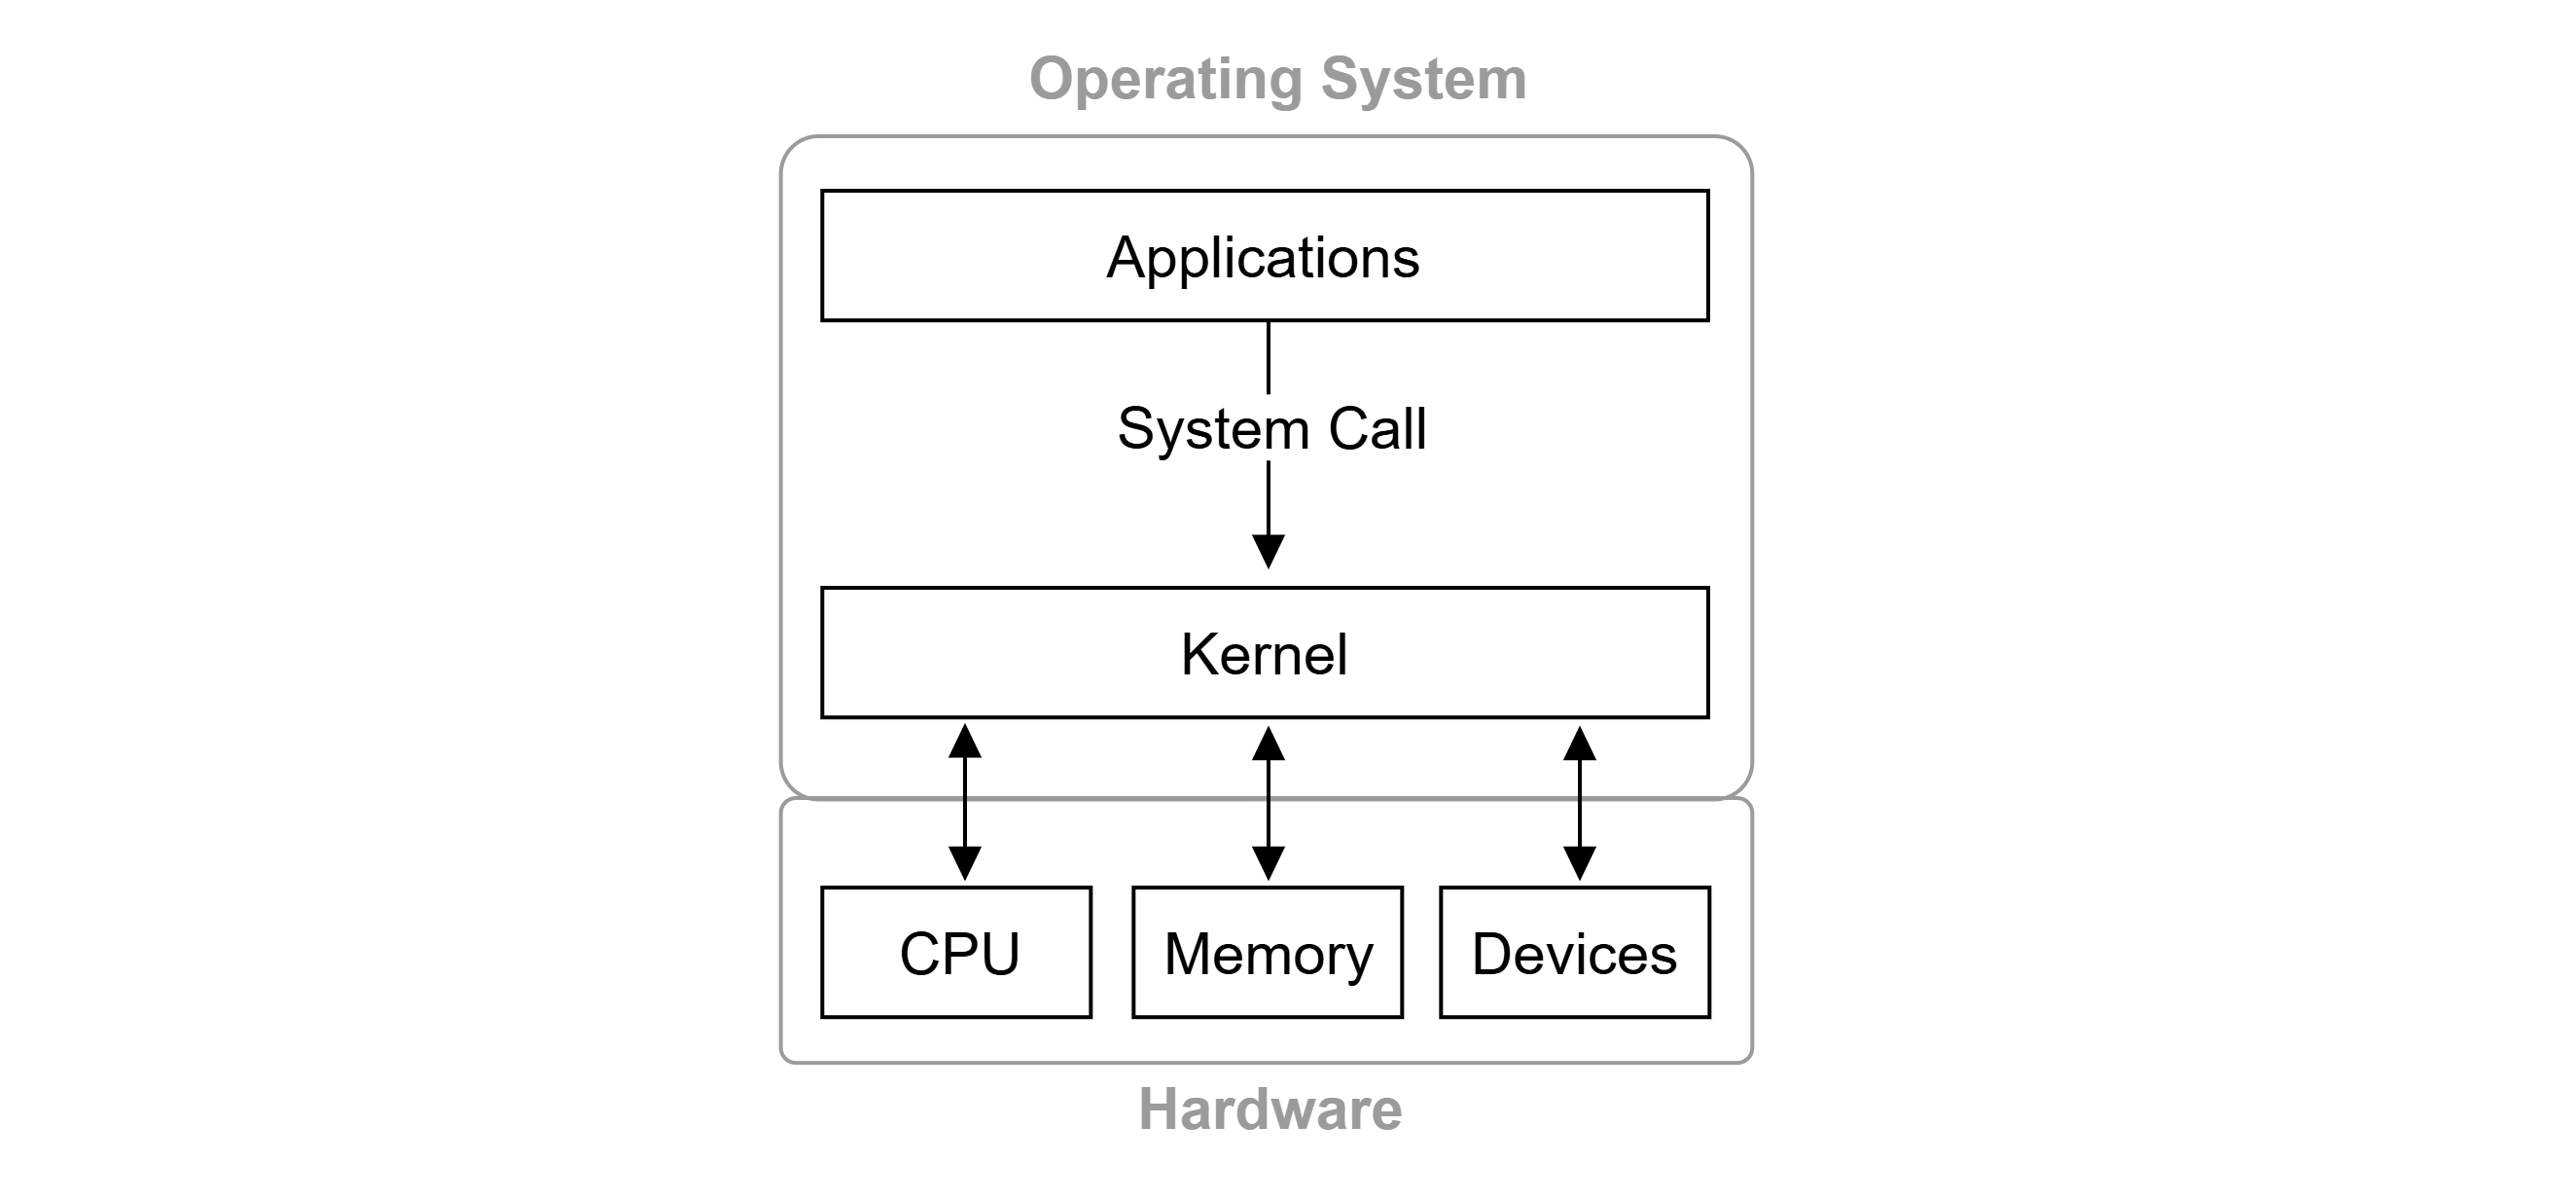
\includegraphics[width=\textwidth]{Sections/cpu/kernel.png}
    \caption{User-level applications make syscalls to the kernel to access hardware resources.}
    \label{fig:kernel}
\end{figure}

\newpage

\begin{Def}[Bus]

    A \textbf{bus} is a collection of physical signal lines (wires or pins) and protocols that carry data, addresses, and control signals between 
    components inside a computer (e.g.\ CPU, memory, I/O devices) or between multiple boards and peripherals. There are two main types of buses:
    \begin{itemize}
        \item \textbf{Serial Bus:} Transfers data one bit at a time over a single channel (e.g., USB).
        \item \textbf{Parallel Bus:} Transfers multiple bits simultaneously over multiple channels (e.g., PCI).
    \end{itemize}
\end{Def}

\begin{Def}[Device Drivers]

  The kernel exposes generic interfaces to various sub-systems (e.g., file system) that user processes can use to perform tasks; \textbf{Device drivers} implement such interfaces,
  translating generic system calls into hardware-specific operations for specific devices (e.g., disk drives, network cards, etc.). Drivers must be loaded into kernel space.
\end{Def}

\noindent
This text does not concern assembly code, so \underline{\textbf{do not}} get caught in the specifics of this Example: 
\begin{Example}[Assembly Code]

    \label{ex:assembly_code}
    An assembly example demonstrating initialized (.data) and uninitialized (.bss) data sections:

    \begin{lstlisting}[language={[x86masm]Assembler}, numbers=none]
    section .data               ; Initialized data section
        num1    dd  7           ; num1 is initialized to 7
        num2    dd  3           ; num2 is initialized to 3

    section .bss                ; Uninitialized data section
        temp    resd 1          ; temp is reserved (uninitialized)
        result  resd 1          ; result is reserved (uninitialized)

    section .text               ; Code section
        global _start

    _start:
        mov eax, [num1]         ; Load num1 into eax
        mov [temp], eax         ; Store num1 in temp
        mov ebx, [num2]         ; Load num2 into ebx
        add eax, ebx            ; Add num2 to eax (eax = num1 + num2)
        mov [result], eax       ; Store the sum in result
    ; Exit syscall removed for simplicity
    \end{lstlisting}

    \noindent
    In this example, `num1' and `num2' are initialized before execution, while `temp' and `result' are uninitialized and only receive values during program execution.
\end{Example}

\newpage 
\section{Code Security}

At a \emph{very} high-level, vulnerabilities exploited by hackers stem from flaws that the programmer forgot to consider (i.e., bugs).
To learn more on cybersecurity, consider our other text \underline{\href{https://github.com/Concise-Works/Cyber-Security/blob/main/main.pdf}{here}}.

\begin{Def}[Proper Encapsulation]

    \label{def:proper_encapsulation}

    \textbf{Proper encapsulation} is the practice of hiding implementation details and exposing only necessary interfaces to prevent unauthorized access or modification.
\end{Def}
\begin{Example}[Student Class]

    \label{ex:student_class}

    Consider a simple `Student' class in an object-oriented programming language:

    \begin{lstlisting}[language=Java, numbers=none]
    public class Student {
        private String name; // Private field, not accessible outside the class
        private int age;     // Private field, not accessible outside the class

        public Student(String name, int age) {
            this.name = name;
            this.age = age;
        }

        public String getName() { // Public method to access name
            return name;
        }
        // Other methods...
    }
    \end{lstlisting}
    Upon creating a new student instance \texttt{new Student("Alice", 20)}, the name and age are private, preventing direct access via \textbf{dot notation} (e.g., \texttt{student.name}).
    The only way to access the name is through the public method \texttt{getName()}. Here we do not have a method for accessing age.
\end{Example}

\begin{Def}[Risks of Accessing Main Memory]

    \label{def:accessing_main_memory}

    Programs accesses main memory (RAM) to read and write data; \textbf{It's critical} that 
    such \underline{references to RAM are abstracted} to avoid malicious or accidental access of data.

    For example, in Java when users print objects, instead of 
    printing the object's memory address, it prints the \texttt{toString()} method, which \textbf{by default} prints the class name and hash code of the object.
\end{Def}
\noindent
In conclusion, there are significant risks when dealing with memory management.